%% ICASSP manuscript (Draft 16) on the official ICASSP 2027 template.
%% Camera-ready revision after the fourth ICASSP review.
%% Figures are intentionally NOT generated in this draft. The boxes reserve the intended final
%% footprint, and detailed figure-generation specifications appear as TeX comments in draft16_2.tex.
%% draft16-camera-ready
\documentclass{article}
\usepackage{spconf,amsmath,amssymb,graphicx,booktabs,array,multirow,url,cite}

\newcommand{\ci}[2]{[{#1},\,{#2}]}
\newcommand{\PFT}{P{+}FT}
\emergencystretch=2em
\renewcommand{\topfraction}{0.94}
\renewcommand{\bottomfraction}{0.88}
\renewcommand{\textfraction}{0.05}
\renewcommand{\floatpagefraction}{0.78}
\setcounter{topnumber}{4}
\setcounter{totalnumber}{5}
\setcounter{dbltopnumber}{3}
\renewcommand{\dbltopfraction}{0.94}
\renewcommand{\dblfloatpagefraction}{0.78}
\setlength{\textfloatsep}{5pt plus 2pt minus 2pt}
\setlength{\floatsep}{6pt plus 2pt minus 2pt}
\setlength{\intextsep}{7pt plus 2pt minus 2pt}
\setlength{\dbltextfloatsep}{5pt plus 2pt minus 2pt}
\setlength{\dblfloatsep}{6pt plus 2pt minus 2pt}
\setlength{\abovecaptionskip}{3pt}
\setlength{\belowcaptionskip}{0pt}

\begin{document}
\ninept

\title{Recovery Gain Is Operating-Point Dependent in Pruned Text-to-Audio Diffusion}

\twoauthors
  {Gabriel Bibb\'o}
  {Independent researcher \\
   \texttt{gabobibbo@gmail.com}}
  {Arshdeep Singh, \, Mark D. Plumbley}
  {King's College London, UK \\
   \{\texttt{arshdeep.singh}, \texttt{mark.plumbley}\}\texttt{@kcl.ac.uk}}

\maketitle

\begin{abstract}
Recovery fine-tuning is usually judged at one inference setting, although the gain it adds may depend on how a compressed generator is used. We study this effect in released AudioLDM-M checkpoints at $65\%$ and $83\%$ pruning using paired generations across duration and prompt domain. At $83\%$ pruning, CLAP recovery rises from $+0.085$ at $3.84$\,s to $+0.244$ at $10.24$\,s. In a matched $20{,}000$-step intervention, changing the fine-tuning duration from $3.84$ to $10.24$\,s makes the long-minus-short interaction smaller rather than larger, with $\Delta J=-0.035$ \ci{-0.064}{-0.004}. Recovery remains strong on held-out Clotho but is an order of magnitude smaller on hip-hop, where dense anchors remain informative and the duration interaction is unresolved near zero. These results show that recovery gain is operating-point dependent and motivate reporting paired recovery across displaced operating points rather than a single post-fine-tuning score.
\end{abstract}

\begin{keywords}
text-to-audio generation, diffusion models, structured pruning, recovery fine-tuning, evaluation
\end{keywords}

\section{Introduction}
Structured pruning reduces diffusion cost by removing complete channels or blocks from the denoising network. Because that reduction usually damages generation quality, practical compression pipelines add an adaptation stage and judge the resulting checkpoint rather than the pruned model alone. This prune-and-recover pattern is established in image diffusion~\cite{fang2023diffpruning,kim2024bksdm,fang2025tinyfusion} and has recently been applied to AudioLDM~\cite{singh2026pruning}.

The usual benchmark answers whether the compressed checkpoint is competitive under one generation recipe. It does not isolate what recovery added, nor does it show whether that addition survives when the model is used differently. A high final score can reflect a strong pruned starting point, a large fine-tuning improvement, or an adaptation that happens to be favorable under the benchmark conditions.

We therefore treat recovery as a paired effect. For a pruned checkpoint P and its fine-tuned counterpart \PFT{}, recovery gain is the change from P to \PFT{} under the same prompt, noise and inference setting. We call that setting the inference \emph{operating point}. Requested duration is one axis, prompt domain is another, and sampler configuration provides a third. This makes recovery a function to be measured rather than a scalar label attached to the checkpoint.

The distinction matters as text-to-audio evaluation moves beyond single aggregate scores. CLAP remains a standard proxy for prompt alignment~\cite{wu2023clap,huang2023makeanaudio,ghosal2023tango}, while newer benchmarks increasingly test robustness and generalization~\cite{wang2026ttabench}. Compression evaluation has not adopted the same perspective systematically. Recovery is still commonly summarized by one post-fine-tuning score at the operating point used for validation.

We study the released pruned and recovered AudioLDM-M-Full checkpoints of Singh et al.~\cite{singh2026pruning}. The released $10^{6}$-step recovery exhibits a strong duration interaction and selective transfer across prompt domains. We then turn the obvious explanation into a directional prediction. Two checkpoints start from the same pruned model, use the same $20{,}000$-step recipe, and differ only in whether fine-tuning uses $3.84$ or $10.24$\,s examples. Training-duration specialization predicts a larger long-minus-short interaction after the $10.24$\,s fine-tune. The data resolve in the opposite direction.

The contribution is therefore not a new pruning rule. It is a way to qualify what recovery means after compression. We quantify how much the recovery increment changes with duration and domain, test one mechanism with a matched intervention, and use dense, chance and real-data anchors to separate a weak gain from an uninformative metric. The resulting protocol is compact enough for routine evaluation while exposing behavior that one post-recovery score would hide. Expanded results and executable provenance are retained in the companion repository~\cite{bibbo2026repo}.

\section{Background and motivation}
\subsection{Recovery is part of the compression pipeline}
Modern diffusion compression methods increasingly optimize for the model that exists after adaptation. Diff-Pruning combines structural removal with retraining~\cite{fang2023diffpruning}. BK-SDM removes residual and attention blocks and transfers behavior through distillation~\cite{kim2024bksdm}. TinyFusion selects architectures according to their expected post-fine-tuning performance~\cite{fang2025tinyfusion}. In each case, the useful compressed system is defined jointly by what pruning removes and what later adaptation restores.

Singh et al.~\cite{singh2026pruning} apply this pattern to AudioLDM by pruning U-Net channels and fine-tuning the reduced model on AudioCaps for $10^{6}$ steps. Their released checkpoints recover strongly on the reported in-domain metrics. Our question begins after that result. Once recovery is part of the method, how stable is the gain produced by recovery when inference moves away from the operating point at which the checkpoint is normally evaluated?

Fine-tuning gives a reason to expect variation. Adaptation can reshape pretrained representations differently across distributions~\cite{kumar2022finetuning}, and text-to-audio systems are already sensitive to prompt and generation conditions. A post-recovery score therefore mixes final checkpoint quality with the increment added by adaptation at that particular setting. Only the latter can tell us where recovery persists.

\subsection{Making recovery interpretable}
Automatic metrics expose different aspects of generated audio. CLAP measures text-audio alignment~\cite{wu2023clap}. FAD measures distributional distance and is sensitive to sample size and embedding choice~\cite{kilgour2019fad,gui2024fad,chung2025kad}. Human-CLAP~\cite{takano2025humanclap}, PANNs~\cite{kong2020panns} and FineLAP~\cite{li2026finelap} provide complementary views of semantic alignment, event content and temporal grounding.

The important distinction is between the quantities computed from these metrics. The final score $S(\PFT)$ describes the checkpoint delivered to a user. The paired difference $S(\PFT)-S(P)$ describes what fine-tuning added at one operating point. A recovery ratio then asks how much of the available gap from P to an interpretable reference was closed. We keep these quantities separate and use dense generations, shuffled-caption chance and real audio as anchors for scale.
\section{Experimental design}
\subsection{Systems and operating points}
The dense reference is AudioLDM-M-Full~\cite{liu2023audioldm}, with $415.96$\,M U-Net parameters. We study the two released pruning severities from Singh et al.~\cite{singh2026pruning}. Severity~1 retains $145.67$\,M parameters after $65.0\%$ pruning, while severity~2 retains $71.08$\,M after $82.9\%$ pruning. At each severity, P denotes the checkpoint before recovery and \PFT{} the released checkpoint after $10^{6}$ AudioCaps fine-tuning steps. Their paired difference measures what the released recovery stage adds within the pruned architecture. It does not by itself identify an effect caused specifically by pruning.

The primary duration comparison uses $3.84$ and $10.24$\,s. Severity~2 adds $5.12$ and $7.68$\,s, producing a four-point sweep. AudioCaps \textsc{test} supplies the in-domain prompts~\cite{kim2019audiocaps}. Clotho provides a held-out sound-event domain with a different caption distribution~\cite{drossos2020clotho}. A second held-out battery uses hip-hop and rap captions from MusicCaps~\cite{agostinelli2023musiclm}. The main severity~2 AudioCaps analysis uses $192$ prompts, Clotho uses $96$, and the extended hip-hop battery uses $127$.

Generation uses DDIM~\cite{song2021ddim} with $50$ steps, guidance $2.5$ and $\eta=0$. A pre-specified robustness check repeats the severity~2 endpoint comparison with the published DDIM $200$, guidance $3.5$ recipe.

\subsection{Interventions and weight conventions}
The mechanism and boundary checks were frozen before their own generation and scoring. They test explanations of the primary finding but are not part of its original confirmatory family.

The central intervention is symmetric. Starting from the same severity~2 P checkpoint, we fine-tune the full U-Net for $20{,}000$ optimizer updates at either $3.84$ or $10.24$\,s while holding every other training choice fixed. Both runs use AdamW with a constant learning rate of $10^{-4}$, default $\beta$ values $(0.9,0.999)$, weight decay $0.01$, no scheduler and effective batch size $2$. The two resulting checkpoints are evaluated at both durations on the same $192$ prompts with common generation noise. If recovery specializes to its training duration, moving training from $3.84$ to $10.24$\,s should increase the long-minus-short interaction, so
\begin{equation}
\Delta J = J_{10.24}-J_{3.84}>0.
\end{equation}

A reduced dense $2\times2$ repeats this exact $20{,}000$-step recipe from AudioLDM-M-Full. Because the experimental exports are raw weights, we also evaluate the raw released dense checkpoint on the same prompts. Raw and EMA baselines differ by at most about $0.02$ CLAP at either duration, which rules out weight convention as an explanation for the much larger changes after fine-tuning. This dense experiment probes the short adaptation recipe only. It cannot replace the unavailable dense checkpoint after the released $10^{6}$-step recovery, and no lower-learning-rate dense run was performed.

The severity~2 P used for the symmetric intervention is derived from dense EMA weights, whereas both $20{,}000$-step fine-tuned checkpoints are raw exports. This convention mismatch cancels exactly in $\Delta J$. On the dense model at step zero, its duration-dependent offset is $-0.019$ \ci{-0.050}{+0.013}, so we treat the individual $J$ values with this caveat and base the specialization test on their paired difference.

Further checks extend the released recovery to $15.36$\,s on $96$ matched prompts, enlarge severity~1 with a disjoint $96$-prompt sample, split the severity~2 AudioCaps draw into two outcome-blind halves, and complete dense hip-hop anchors for all $127$ prompts. These analyses probe response shape, prompt-sample stability and metric-floor interpretations.

\subsection{Pairing, endpoints and estimands}
Within each operating point, compared checkpoints receive identical diffusion noise $x_T$ for a given prompt. The prompt is the statistical unit, and $95\%$ intervals use a prompt-level percentile bootstrap with $B=10^{4}$ resamples. This common-random-number design makes $R$ a paired effect rather than a difference between independently sampled generation sets.

The primary endpoint is fused CLAP cosine from \texttt{laion/\allowbreak clap-htsat-fused}, revision \texttt{365dea6e}~\cite{wu2023clap}. Human-CLAP provides a second alignment scorer. KL is measured against matched real references, with positive recovery meaning that \PFT{} reduces KL relative to P. For PANNs, \emph{top-10 capture} is the number of ground-truth AudioSet labels from the reference clip that appear among the generated clip's ten highest-scoring PANNs classes. PANNs capture recovery is the paired increase in that count from P to \PFT{}.

For operating point $o$, recovery gain is
\begin{equation}
R(o)=\mathbb{E}_{i}\left[S(\PFT,i,o)-S(P,i,o)\right].
\end{equation}
The duration interaction is $J=R(10.24\,\mathrm{s})-R(3.84\,\mathrm{s})$. We also report
\begin{equation}
\rho_{\mathrm{ref}}=\frac{R}{S(\mathrm{ref})-S(P)},
\end{equation}
which expresses the gain as a fraction of the available gap to a dense or real-audio reference. Because $\rho$ is a ratio of estimated quantities, its interval can be wide when recovery is small or the reference gap is noisy.

% ========================== FIGURE 1 SPECIFICATION ==========================
% IMPORTANT: The following figure is intentionally a layout placeholder. Do not
% replace the reserved boxes with a synthetic graph. Generate the final figure
% from the committed per-prompt result artifacts.
%
% Intended final figure footprint:
%   - one figure* spanning both columns
%   - two side-by-side panels
%   - each plot area exactly about 0.49\textwidth wide and 4.80 cm high
%   - caption below, matching the current placeholder footprint
%
% PANEL (a), operating-point response of the released recovery
%   Scientific purpose:
%     Show the main duration dependence and the uncertainty beyond 10.24 s.
%   X axis:
%     requested duration in seconds: 3.84, 5.12, 7.68, 10.24, 15.36.
%   Y axis:
%     paired CLAP recovery gain R = CLAP(P+FT)-CLAP(P).
%   Main series:
%     severity-2 released 10^6-step recovery at 3.84/5.12/7.68/10.24,
%     n=192, point estimate with 95% prompt-bootstrap CI.
%   Matched extension:
%     plot the n=96 matched-subset point at 10.24 s separately (open marker)
%     and connect THAT point, not the n=192 point, to the 15.36 s n=96 result
%     with a dashed segment. This visually respects the paired D4 comparison.
%   Annotation:
%     D4 = R(15.36)-R(10.24 matched) = +0.021 [-0.023,+0.067].
%     Use wording "no clear increase" or only the CI. Do not label plateau.
%   Optional reference cue:
%     a light vertical guide at 10.24 s may mark the native duration, but it
%     must not imply that 10.24 s is a maximum.
%
% PANEL (b), symmetric training-duration intervention
%   Scientific purpose:
%     Make the specialization prediction and its falsification visually obvious.
%   X axis:
%     evaluation duration: 3.84 and 10.24 s.
%   Y axis:
%     20k-step fine-tuning gain over the SAME severity-2 P baseline.
%   Series 1:
%     shortft, trained at 3.84 s, R at both evaluation durations with 95% CIs.
%   Series 2:
%     longft, trained at 10.24 s, R at both evaluation durations with 95% CIs.
%   Annotate or bracket the two slopes:
%     J_short = +0.065 [+0.044,+0.087]
%     J_long  = +0.031 [+0.010,+0.052]
%     Delta J = J_long-J_short = -0.035 [-0.064,-0.004].
%   Visual logic:
%     specialization predicts the long-trained line should have a larger
%     long-minus-short slope. The observed ordering is the opposite.
%   Do NOT add the dense 2x2 or public dense text-FT reference to this panel.
%     They answer different questions and would obscure the matched comparison.
%   Styling:
%     simple point-lines with vertical 95% CI whiskers, no decorative shading,
%     direct labels or a small legend, readable at two-column ICASSP print size.
% ===========================================================================
\begin{figure*}[t]
\centering
\begin{minipage}[t]{0.49\textwidth}
\centering
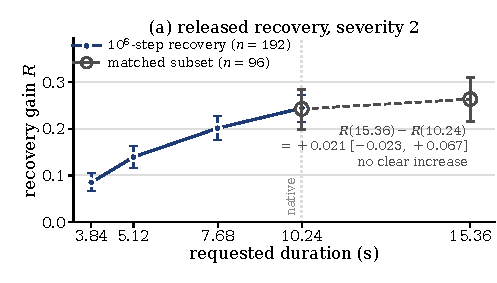
\includegraphics[width=0.965\linewidth]{fig1a_duration.pdf}
\end{minipage}\hfill
\begin{minipage}[t]{0.49\textwidth}
\centering
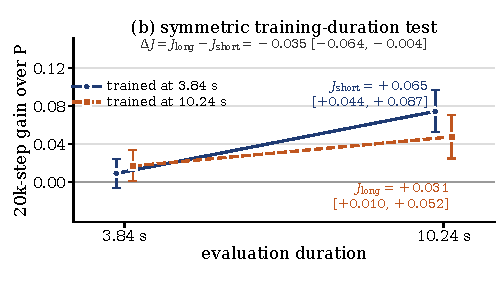
\includegraphics[width=0.965\linewidth]{fig1b_intervention.pdf}
\end{minipage}
\caption{Duration dependence and the symmetric training-duration test. Left, the released severity~2 recovery is evaluated across duration, with the $15.36$\,s extension compared on its matched $96$-prompt subset. Right, two $20{,}000$-step fine-tunes from the same pruned checkpoint differ only in training duration and are evaluated at both $3.84$ and $10.24$\,s.}
\label{fig:duration}
\end{figure*}
\section{Results}
\subsection{Recovery changes with requested duration}
The released severity~2 recovery shows a large duration interaction. CLAP gain rises from $R=+0.085$ \ci{+0.066}{+0.105} at $3.84$\,s to $+0.244$ \ci{+0.215}{+0.273} at $10.24$\,s, giving $J=+0.159$ \ci{+0.131}{+0.187}. The intermediate points in Table~\ref{tab:evidence} show a gradual response rather than an endpoint anomaly. The scale also changes materially. Recovery closes $44\%$ of the gap from P to dense at $3.84$\,s and $82\%$ at $10.24$\,s.

Human-CLAP, KL to matched real references and PANNs top-10 capture all support larger recovery as duration increases, but they do not imply continued growth at every step. Human-CLAP is essentially saturated by $7.68$\,s, changing only from $0.371$ to $0.375$ recovery at $10.24$\,s. The published DDIM $200$, guidance $3.5$ recipe still reproduces the endpoint interaction with $J=+0.184$ \ci{+0.126}{+0.243}, and the registered severity~2 conclusions survive Holm correction. These checks reuse the AudioCaps prompt draw, so they establish metric and sampler robustness rather than an independent prompt replication.

Extending generation beyond the native duration does not reveal a sharp peak. On the matched $96$-prompt subset, recovery changes by $+0.021$ \ci{-0.023}{+0.067} from $10.24$ to $15.36$\,s. The interval is too wide to establish a plateau, but it provides no clear evidence of another increase comparable with the earlier sweep steps.

\subsection{Training duration does not determine the favorable evaluation duration}
The matched $20{,}000$-step intervention supplies the direct test. The checkpoint trained at $3.84$\,s has $J_{3.84}=+0.065$ \ci{+0.044}{+0.087}; the checkpoint trained at $10.24$\,s has the smaller interaction $J_{10.24}=+0.031$ \ci{+0.010}{+0.052}. Their paired difference is $\Delta J=-0.035$ \ci{-0.064}{-0.004}. Training-duration specialization predicts the opposite sign because moving training to $10.24$\,s should increase the long-minus-short advantage. At this matched budget, the favorable evaluation duration therefore does not follow the duration used for fine-tuning.

The dense $2\times2$ gives a clean negative result for this particular training recipe. Raw and EMA dense baselines differ by only $+0.001$ \ci{-0.017}{+0.020} at $3.84$\,s and $-0.017$ \ci{-0.044}{+0.010} at $10.24$\,s, whereas every $20{,}000$-step dense gain is strongly negative, between $-0.220$ and $-0.168$ with upper $95\%$ bounds below $-0.144$. Its training-duration contrast is nevertheless unresolved, $\Delta J_{\rm dense}=-0.005$ \ci{-0.033}{+0.025}. The quantity is measurable, but it is not a clean analogue of recovery because both dense runs have entered a degraded regime under AdamW at $10^{-4}$. A smaller learning rate might avoid this regime, but that hypothesis was not tested.

A public dense text-fine-tuned checkpoint trained with a different recipe provides a separate reference. Its gain is $-0.022$ \ci{-0.061}{+0.017} at $3.84$\,s and $+0.091$ \ci{+0.042}{+0.141} at $10.24$\,s, giving $J=+0.113$ \ci{+0.051}{+0.173}. Because the recipe and training history are not matched, this result is supporting context rather than a causal control.

\begin{table*}[t]
\centering
\caption{Recovery across duration and domain. All intervals are $95\%$ prompt-bootstrap intervals. Positive KL recovery means that \PFT{} reduces KL to the matched real reference relative to P. Human-CLAP, KL and PANNs sweep rescoring are corroborative analyses.}
\label{tab:evidence}
\setlength{\tabcolsep}{4.0pt}
\begin{tabular}{@{}lcccc@{}}
\toprule
Duration & CLAP $R$ & Human-CLAP $R$ & KL recovery & PANNs capture $R$ \\
\midrule
$3.84$ s & $.085$ $[.066,.105]$ & $.189$ $[.162,.217]$ & $.66$ $[.43,.92]$ & $.19$ $[.06,.32]$ \\
$5.12$ s & $.139$ $[.115,.164]$ & $.278$ $[.243,.314]$ & $1.16$ $[.91,1.41]$ & $.38$ $[.23,.53]$ \\
$7.68$ s & $.201$ $[.175,.227]$ & $.371$ $[.336,.405]$ & $1.95$ $[1.68,2.23]$ & $.76$ $[.61,.91]$ \\
$10.24$ s & $.244$ $[.215,.273]$ & $.375$ $[.340,.409]$ & $2.22$ $[1.92,2.52]$ & $.86$ $[.70,1.02]$ \\
$J$ & $.159$ $[.131,.187]$ & $.185$ $[.151,.220]$ & $1.56$ $[1.20,1.92]$ & $.67$ $[.49,.85]$ \\
\midrule
Domain & $n$ & $R(3.84\,\mathrm{s})$ & $R(10.24\,\mathrm{s})$ & $\rho_{\rm dense}(10.24\,\mathrm{s})$ \\
\midrule
AudioCaps & 192 & $.085$ $[.066,.105]$ & $.244$ $[.215,.273]$ & $.82$ \\
Clotho & 96 & $.098$ $[.072,.125]$ & $.210$ $[.176,.243]$ & $.74$ \\
Hip-hop & 127 & $.026$ $[.007,.044]$ & $.027$ $[.003,.050]$ & $.119$ $[.015,.215]$ \\
\bottomrule
\end{tabular}
\end{table*}

\subsection{Duration dependence weakens where recovery is weak}
Clotho shows that leaving AudioCaps does not by itself remove recovery. At $10.24$\,s, Clotho gives $R=+0.210$ \ci{+0.176}{+0.243} and closes $74\%$ of the dense gap. Its duration interaction remains substantial, $J=+0.112$ \ci{+0.079}{+0.146}. The difference from the AudioCaps interaction is $+0.047$ \ci{+0.003}{+0.090}.

Hip-hop behaves differently. With all $127$ prompts, recovery stays near $+0.03$ at both durations and its interaction is $J=+0.001$ \ci{-0.026}{+0.028}. Dense alignment remains about $+0.11$ above shuffled-caption chance, so the small gain is not caused by a floor-limited battery. Recovery closes about $12\%$ of the native dense gap, but this ratio is imprecise because both its small numerator and estimated denominator contribute uncertainty. Across the three domains, the duration interaction is largest where recovery itself is largest, intermediate on Clotho, and unresolved near zero on hip-hop. This connects the duration and domain effects rather than treating them as independent phenomena.

\subsection{Prompt-sample and short-generation diagnostics}
Severity~1 shows genuine prompt-set heterogeneity. The original outcome-blind $80$-prompt draw gives $J=+0.044$ \ci{-0.000}{+0.088}, whereas a disjoint $96$-prompt draw gives $+0.169$ \ci{+0.115}{+0.222}; their difference is $+0.124$ \ci{+0.058}{+0.194}. Both draws were selected without outcomes, but the second used a different seeded-hash salt and required five caption rows per clip, so they are not identical sampling rules. Severity~2 is much more stable under the same diagnostic. Its two outcome-blind $96$-prompt halves give $J=+0.159$ \ci{+0.116}{+0.200} and $+0.160$ \ci{+0.122}{+0.198}, with a difference of $+0.001$ \ci{-0.056}{+0.057}. Clotho supplies an additional independent prompt set on which the interaction also resolves.

Under CLAP, base-model degradation at $3.84$\,s does not account for the interaction. The dense model's floor-corrected response from $3.84$ to $10.24$\,s is $+0.142$ \ci{+0.111}{+0.172}, close to the real-audio crop response of $+0.150$ \ci{+0.133}{+0.166}. This is scorer-internal evidence rather than a perceptual claim. A separate crop analysis shows that recovery itself still depends on how the clip is generated. Scoring the first $3.84$\,s of a $10.24$\,s generation gives $R_{\rm crop}=+0.172$ \ci{+0.150}{+0.194}, which is $+0.087$ \ci{+0.065}{+0.110} above recovery from a separately generated $3.84$\,s clip.
\section{Discussion and limitations}
The central result is that recovery gain depends on the operating point, not that one training duration is intrinsically preferred. The symmetric intervention makes this distinction falsifiable. Specialization predicts that moving fine-tuning from $3.84$ to $10.24$\,s should increase the long-minus-short recovery interaction. Instead, both fine-tunes gain more at the longer evaluation duration and the interaction becomes smaller after training at $10.24$\,s.

A useful working hypothesis is therefore that fine-tuning changes the model in ways whose measurable benefit is expressed differently across inference conditions. The domain results support that interpretation at a descriptive level. AudioCaps shows the largest recovery and duration interaction, Clotho retains much of both, and hip-hop shows weak recovery with essentially no duration interaction. The public dense text-fine-tuned reference also favors the longer evaluation duration, although it is not recipe-matched. These observations do not identify a mechanism, but they argue against treating duration dependence as a simple memory of the training duration.

The dense diagnostics sharpen the causal boundary. Raw and EMA baselines differ by at most about $0.02$ CLAP, yet AdamW at $10^{-4}$ for $20{,}000$ steps drives every dense gain below $-0.16$ while improving the pruned checkpoint. We did not test a smaller learning rate, so an overly aggressive update for an already converged dense model remains a plausible explanation. The experiment therefore characterizes this short recipe, not dense recovery in general, and it cannot replace the unavailable dense checkpoint after the released $10^{6}$-step recovery.

The remaining limits concern generality and measurement. The study covers one model family, two pruning severities and a small domain grid. Severity~1 is sensitive to prompt selection, although the severity~2 split-half analysis is stable and Clotho independently reproduces a positive duration interaction. The step from $10.24$ to $15.36$\,s is too uncertain to establish a plateau. The argument that short-duration base behavior does not explain the interaction is limited to CLAP and should not be read as a perceptual claim. Human-CLAP, KL and PANNs provide corroboration, but the small author listening exercise remains descriptive only.

The practical implication is simple. A recovery claim should report the paired increment from P to \PFT{} at the intended operating point and at deliberately displaced points. Common generation noise improves precision, while dense, chance or real-data anchors make the scale interpretable. If a mechanism is proposed, the most informative next experiment is one that changes its directional prediction. Here, matching the fine-tuning budget while changing only training duration was more informative than another aggregate score.

\section{Conclusion}
Recovery fine-tuning gain is strongly operating-point dependent in the AudioLDM-M checkpoints studied here. The duration interaction is robust at severity~2 and appears on an independent Clotho prompt set, while a symmetric intervention shows that it does not follow training duration at a matched $20{,}000$-step budget. Recovery remains strong on Clotho but weak on hip-hop, where the duration interaction also disappears despite informative dense anchors. Reporting recovery as a paired function of operating point therefore gives a more faithful account of compressed-model behavior than a single post-fine-tuning score.

\clearpage
{\setlength{\itemsep}{0pt}\setlength{\parsep}{0pt}
\begin{thebibliography}{99}
\bibitem{fang2023diffpruning} G.~Fang, X.~Ma, and X.~Wang, ``Structural pruning for diffusion
models,'' in \emph{Proc.\ NeurIPS}, 2023.
\bibitem{kim2024bksdm} B.-K.~Kim, H.-K.~Song, T.~Castells \emph{et al.}, ``BK-SDM: A lightweight, fast,
and cheap version of Stable Diffusion,'' in \emph{Proc.\ ECCV}, 2024.
\bibitem{fang2025tinyfusion} G.~Fang, K.~Li, X.~Ma, and X.~Wang, ``TinyFusion: Diffusion transformers
learned shallow,'' in \emph{Proc.\ CVPR}, 2025.
\bibitem{liu2023audioldm} H.~Liu, Z.~Chen, Y.~Yuan \emph{et al.}, ``AudioLDM: Text-to-audio generation with latent diffusion models,'' in
\emph{Proc.\ ICML}, 2023.
\bibitem{singh2026pruning} A.~Singh, Y.~Yuan, Y.~Chen, W.~Wang, and M.~D.~Plumbley, ``Efficient
text-to-audio generation via pruning,'' arXiv:2607.13330, 2026.
\bibitem{wu2023clap} Y.~Wu, K.~Chen, T.~Zhang \emph{et al.},
``Large-scale contrastive language-audio pretraining with feature fusion and keyword-to-caption
augmentation,'' in \emph{Proc.\ ICASSP}, 2023.
\bibitem{huang2023makeanaudio} R.~Huang, J.~Huang, D.~Yang \emph{et al.}, ``Make-An-Audio:
Text-to-audio generation with prompt-enhanced diffusion models,'' in \emph{Proc.\ ICML}, 2023.
\bibitem{ghosal2023tango} D.~Ghosal, N.~Majumder, A.~Mehrish, and S.~Poria, ``Text-to-audio generation
using instruction guided latent diffusion model,'' in \emph{Proc.\ ACM Int.\ Conf.\ Multimedia (MM)},
2023, pp.~3590--3598.
\bibitem{kilgour2019fad} K.~Kilgour, M.~Zuluaga, D.~Roblek \emph{et al.}, ``Fr\'echet Audio
Distance: A reference-free metric for evaluating music enhancement algorithms,'' in
\emph{Proc.\ Interspeech}, 2019.
\bibitem{gui2024fad} A.~Gui, H.~Gamper, S.~Braun \emph{et al.}, ``Adapting Fr\'echet Audio
Distance for generative music evaluation,'' in \emph{Proc.\ ICASSP}, 2024.
\bibitem{chung2025kad} Y.~Chung, P.~Eu, J.~Lee \emph{et al.}, ``KAD: No more FAD!
An effective and efficient evaluation metric for audio generation,'' arXiv:2502.15602, 2025.
\bibitem{kong2020panns} Q.~Kong, Y.~Cao, T.~Iqbal \emph{et al.}, ``PANNs:
Large-scale pretrained audio neural networks for audio pattern recognition,'' \emph{IEEE/ACM
Trans.\ Audio, Speech, Lang.\ Process.}, vol.~28, pp.~2880--2894, 2020.
\bibitem{takano2025humanclap} T.~Takano, Y.~Okamoto, Y.~Kanamori \emph{et al.}, ``Human-CLAP:
Human-perception-based contrastive language-audio pretraining,'' in \emph{Proc.\ APSIPA ASC}, 2025,
pp.~131--136.
\bibitem{li2026finelap} X.~Li, X.~Xu, Z.~Ma \emph{et al.}, ``FineLAP: Taming
heterogeneous supervision for fine-grained language-audio pretraining,'' in \emph{Proc.\ ACL}, 2026,
pp.~10393--10408.
\bibitem{kumar2022finetuning} A.~Kumar, A.~Raghunathan, R.~Jones \emph{et al.}, ``Fine-tuning
can distort pretrained features and underperform out-of-distribution,'' in \emph{Proc.\ ICLR}, 2022.
\bibitem{kim2019audiocaps} C.~D.~Kim, B.~Kim, H.~Lee, and G.~Kim, ``AudioCaps: Generating captions
for audios in the wild,'' in \emph{Proc.\ NAACL-HLT}, 2019.
\bibitem{drossos2020clotho} K.~Drossos, S.~Lipping, and T.~Virtanen, ``Clotho: An audio captioning dataset,'' in \emph{Proc.\ ICASSP}, 2020.
\bibitem{agostinelli2023musiclm} A.~Agostinelli, T.~I.~Denk, Z.~Borsos \emph{et al.}, ``MusicLM:
Generating music from text,'' arXiv:2301.11325, 2023.
\bibitem{song2021ddim} J.~Song, C.~Meng, and S.~Ermon, ``Denoising diffusion implicit models,'' in
\emph{Proc.\ ICLR}, 2021.
\bibitem{wang2026ttabench} H.~Wang, C.~Liu, J.~Chen \emph{et al.}, ``TTA-Bench: A comprehensive benchmark for evaluating text-to-audio models,'' in \emph{Proc.\ AAAI}, 2026, pp.~33512--33520.
\bibitem{bibbo2026repo} G.~Bibb\'o, A.~Singh, and M.~D.~Plumbley, ``Companion repository for operating-point evaluation of recovery fine-tuning,'' 2026. [Online]. Available: \url{https://github.com/gbibbo/audioldm-modality-swap-pruning/tree/main/paper-operating-point-recovery}
\end{thebibliography}}

\end{document}
